\section{Mikrokontroler ATmega8535}

	\subsection{Mikrokontroler}
		Mikrokontroler adalah komponen elektronik yang berisikan rangkaian mikroprosesor, memori (RAM/ROM) dan I/O, rangkaian tersebut terdapat dalam level chip atau yang biasa disebut single chip mikrokomputer. Pada mikrokontroler sudah ada komponen-komponen mikroprosesor dengan beberapa bus internal yang saling berhubungan. Komponen – komponen tersebut adalah RAM, ROM, Timer, I/O paralel, serial, dan interrupt controller. Dikarenakan harganya yang terjangkau, mikrokontroler ini pun digunakan pada banyak sistem elektronik, seperti di robot, sistem alarm, peralatan telekomunikasi, sampai ke sistem automasi industri.
		
	\subsection{Chipset ATMEGA 8535}
		Mikrokontroler sebagai sebuah \"one chip solution\" dasarnya adalah rangkaian yang terintregrasi (Integrated Circuit-IC) yang secara lengkap mengandung banyak komponen yang membentuk sebuah komputer. Berbeda halnya dengan menggunakan mikroprosesor yang memerlukan komponen luar tambahan seperti RAM, ROM, Timer, dan lain - lain untuk sistem mikrokontroler, komponen - komponen diatas hampir tidak perlu ditambahkan lagi. Karena semua komponen - komponen penting diatas sudah ditanam bersamaan dengan sistem prosesor ke dalam IC tunggal mikrokontroler tersebut. Karena hal tersebut sistem mikrokontroler biasa disebut dengan istilah the real Computer On a Chip (komputer utuh dalam kepingan tunggal), sedangkan sistem mikroprosesor biasa disebut dengan istilah yang terbatas yaitu Computer On a Chip (komputer dalam kepingan tunggal).
		Arsitektur yang digunakan oleh mikrokontroler AVR adalah RISC 8 bit, yang instruksinya dibungkus atau dikemas dalam kode 16-bit dan hampir setiap instruksi dieksekusi dalam 1 siklus clock, hal ini berbeda dengan instruksi MCS51 yang membutuhkan 12 siklus clock. Itu terjadi karena kedua jenis mikrokontroler tersebut memiliki arsitektur yang berbeda. Teknologi yang digunakan AVR adalah RISC (Reduced Instruction Set Computing), sedangkan seri MCS51 berteknologi CISC (Complex Instruction Set Computing). Umumnya ada empat kelompok AVR , yaitu AT90Sxx, ATMega, ATtiny dan AT86RFxx. Pada dasarnya yang membedakan setiap kelas adalah memorinya, peripheralnya dan fungsinya. Dari segi arsitektur dan instruksi yang digunakan, mereka dapat dikatakan hampir sama.
		
		\subsection{Konfigurasi Pin ATmega8535}
		 Kita dapat melihat konfigurasi pin ATmega8535 pada gambar 2.6, Dari gambar itu dapat dijelaskan secara fungsinya konfigurasi pin ATmega8535 sebagai berikut :
		\begin{itemize}
			\item VCC adalah pin yang digunakan untuk memasukan catu daya.
			\item GND madalah pin ground.
			\item Port A (PA0..PA7) adalah pin I/O dua arah dan pin masukan ADC.
			\item Port A (PA0..PA7) adalah pin I/O dua arah dan pin masukan ADC.
			\item Port C (PC0..PC7) adalah pin I/O dua arah dan pin fungsi khusus, yaitu TWI, komparator analog dan Timer Oscilator.
			\item Port D (PD0..PD7) merupakan pin I/O dua arah dan pin fungsi khusus, yaitu komparator analog, interupsi eksternal dan komunikasi serial.
			\item RESET adalah pin yang fungsinya untuk me-reset mikrokontroler.
			\item XTAL1 dan XTAL2 adalah pin masukan clock eksternal.
			\item AVCC adalah pin masukan tegangan untuk ADC.
			\item AREF adalah pin masukan tegangan referensi ADC.
		\end{itemize}

\section{ATmega8}

	\subsection{Penjelasan}
		
		\begin{figure}[ht]
			\centerline{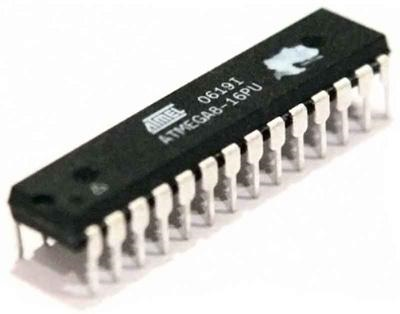
\includegraphics[width=0.5\textwidth]{figures/atmega8.jpg}}
			\caption{Gamber Atmega}
			\label{atmega8}
			\end{figure}
			
		Sekarang kami akan membahas tentang ATMega8. Kami akan membahas tentang fungsi pin, clock, fuse bit, dll. mikrokontroler ATMega8 merupakan mikrokontroler keluarga AVR 8bit. Beberapa tipe mikrokontroler yang satu jenis dengan ATMega8 ini adalah ATMega8535, ATMega16, ATMega32, ATmega328, dll. Yang membedakan antara mikrokontroler yang tadi adalah, ukuran memori, banyaknya GPIO (pin input/output), peripherial (USART, timer, counter, dll).Dari segi ukuran fisik, ATMega8 memiliki ukuran yang lebih kecil dari pada mikrokontroler yang telah disebutkan diatas. Tetapi walaupun ukurannya kecil ATMega8 tidak kalah dengan yang lainnya karena ukuran memori dan bagian lainnya relatif sama dengan ATMega32, ATMega8535, atau yang lainnya. Hanya saja jumlah GPIO nya lebih sedikit dibandingkan mikrokontroler yang telah disebutkan. Untuk penjelasan lebih lanjut akan dibahas di bawah ini.
	
	\subsection{Fungsi dan Kebutuhan Pin}
	
		\begin{figure}[ht]
			\centerline{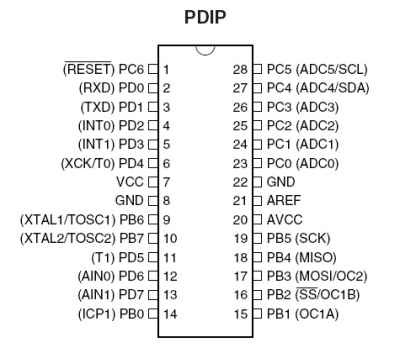
\includegraphics[width=0.5\textwidth]{figures/pdip.jpg}}
			\caption{PDIP}
			\label{pdip}
			\end{figure}
			
		Pinout dari IC mikrokontroler ATMega8 yang berpackage DIP dapat dilihat di bawah ini.
		Dari gambar yang kita lihat dapat kita simpulkan bahwa ada 3 PORT utama dari ATMega8 yaitu PORTB, PORTC, dan PORTD dengan jumlah seluruh pin input/output nya sebanyak 23 pin. PORT tersebut berfungsi sebagai input/output digital atau juga berfungsi sebagai periperial lainnya.
		
	\subsection{Mikrokontroler ATmega8}
	
		\begin{figure}[ht]
			\centerline{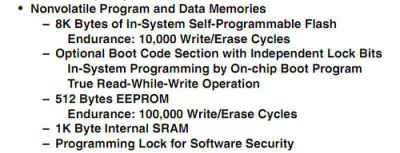
\includegraphics[width=0.5\textwidth]{figures/datamemori.jpg}}
			\caption{Datasheet}
			\label{datamemori}
			\end{figure}
			
		ATMega8 adalah mikrokontroler keluarga AVR 8 bit yang biasa digunakan oleh pemula. Seperti yang terbaca, mikrokontroler ini mempunyai flash memori yang berukuran sebesar 8KB, SRAM yang berukuran sebesar 1KB, dan memori EEPROM sebesar 512 Bytes. Dibawah ini akan di jelaskan sedikit tentang perbedaan dari ketiga itu.
	\subsection{Jenis dan ukuran memori ATmega8}
		Flash memori adalah tempat dimana kita  menyimpan program yang kita buat. Setelah kita mengompilasi program, kita akan mendapatkan file hex yang akan dimasukkan ke dalam  mikrokontroler. File hex itu nantinya akan disimpan di memori yang disebut flash memori. Saat melakukan proses pemograman (coding), biasanya kita memerlukan sesuatu yang disebut dengan variabel atau tempat menampung data.
		Saat mikrokontroler menjalankan suatu program, terdapat proses yang melibatkan variabel (seperti aritmatika). Maka data dari variabel tersebut akan disimpan di memori yang bernama SRAM. Lalu jika ingin menyimpan data seperti halnya pada flashdisk (data tidak hilang ketika tidak ada aliran listrik), kita dapat menyimpannya pada sebuah memori yang bernama EEPROM. EEPROM mirip dengan hardisk, flashdisk yang biasa digunakan pada komputer yaitu sebagai tempat penyimpanan data yang tidak terpengaruh terhadap aliran listrik.
	\subsection{Kebutuhan supply ATMega8}
	
		\begin{figure}[ht]
			\centerline{\includegraphics[width=0.5\textwidth]{figures/sebelum.jpg}}
			\caption{VOLTASE}
			\label{voltase}
			\end{figure}
			
		Sekarang kita masuk ke kebutuhan supply. Di dalam datasheet tertulis seperti pada gambar dibawah ini:
		Didalam gambar tersebut tertulis \"operating voltages 2.7 – 5.5 volt (ATMega8L)\" dan \"4.5 – 5.5 volt (ATMega8).)\". Dan di situ terdapat dua jenis operating voltages, yang pertama adalah untuk ATMega8L dan  yang kedua adalah untuk ATMega8. ATMega8 dan ATMega8L dapat dikatakan sama, tetapi terdapat beberapa perbedaan diantara keduanya, yaitu  jika kita ingin mengaplikasikan sesuatu yang membutuhkan suplly tegangan rendah atau low voltages maka kita akan menggunakan ATMega8L. Karena pada ATMega8L operating voltagenya adalah antara 2.7-5.5 volt.
		Selain itu juga, frekuensi maksimal yang dapat digunakan pada ATMega8L hanya sebesar 8MHz, berbeda dengan ATMega8 yang frekuensi maksimalnya sebesar 16MHz. Jika minimum system yang akan kalian buat nanti menggunakan mikrokontroler ATMega8 maka kalian akan menggunakan tegangan suplly dari 4.5 – 5.5 volt.

\section{ATMega16}
		AVR ATMega16 adalah mikrokontroler CMOS 8-bit yang dibuat oleh Atmel, yang basisnya adalah arsitektur RISC atau Reduced Instruction Set Computer. Hampir semua instruksinya dieksekusi dalam satu siklus clock. AVR mempunyai 32 register general-purpose, timer/counter fleksibel dengan mode compare, interrupt internal dan eksternal, serial UART, programmable Watchdog Timer, dan mode power saving, ADC dan PWM internal. Di dalam AVR terdapat sesuatu yang dinamakan In-System Programmable Flash on-chip yang berfungsi untuk memrogram ulang memori program dalam sistem menggunakan hubungan serial SPI. ATMega16. ATMega16 mempunyai throughput mendekati 1 MIPS per MHz membuat disainer sistem untuk mengoptimasi konsumsi daya versus kecepatan proses.
	\subsection{Pembagian Kelas ATMega16}
		AVR dibagi lagi menjadi empat kelas, yaitu AT902xx, Attiny, AT86RFxx, dan Atmega. Umumnya yang membedakan setiap kelas adalah memorinya, peripheral, dan fungsinya. Silahkan buka website official dari atmel  untuk informasi yang lebih lanjut dalam hal berbagai variasi AVR. Kalian juga dapat mencoba Atmega8, Attiny2313 dengan ukuran Flash Memory 2KB dengan dua input analog, untuk mikrokontroler AVR yang berukuran lebih kecil.
	\subsection{Peta Memori ATMega16}
		Memori Program dari ATMega16 mempunyai dua memori utama, yaitu memori data dan memori program. Selain itu, ATMega16 memiliki memori EEPROM untuk menyimpan data. Untuk menyimpan program ATMega16 memiliki 16K byte On-chip In-System Reprogrammable Flash Memory. Semua instruksi ATMega16 memiliki format 16 atau 32 bit, karna itu memori flash diatur dalam 8K x 16 bit. Memori flash dibagi lagi kedalam dua bagian, yaitu bagian program boot dan bagian aplikasi. Bootloader adalah program kecil yang bekerja pada saat sistem dimulai atau biasa disebut booting yang dapat memasukkan seluruh program aplikasi ke dalam memori prosesor.
	\subsection{Memori Data ATMega16}
		 Ada 3 bagian dari memori data ATMega16, yaitu 32 register umum, 64 buah register I/O dan 1 Kbyte SRAM internal. Yang pertama, Register umum menempati alamat data terbawah, yaitu $00 sampai $1F. Yang ke dua, memori I/O bertempat di 64 alamat berikutnya yang dimulai dari $20 hingga $5F dan juga sebagai register yang hanya digunakan untuk mengatur fungsi dari berbagai fitur mikrokontroler seperti timer atau counter, kontrol register, fungsi - fungsi I/O, dan lain - lain.  Yang ke tiga, 1024 alamat berikutnya mulai dari $60 hingga $45F digunakan untuk SRAM internal.
	\subsection{Memori Data EEPROM}
		ATMega16 ini terdiri dari 512 byte memori data EEPROM 8 bit, dari memori ini kita juga dapat menulis atau membaca data, ketika daya dimatikan, data terakhir yang ditulis pada memori EEPROM masih tersimpan pada memori ini, atau dapat dikatakan memori EEPROM ini bersifat nonvolatile. Alamat dari memori EEPROM mulai dari $000 sampai $1FF.
	\subsection{Port ATMega16}
		Terdapat empat buah port di ATMega16, yaitu PortA, PortB, PortC, dan PortD. Keempat port ini merupakan jalur  bidireksional dengan pilihan  internal pull-up. Setiap port mempunyai tiga buah register bit, yaitu DDxn, PORTxn, dan PINxn. Huruf \"x\" mewakili nama huruf dari port sedangkan huruf \"n\" mewakili nomor bit. Di I/O address DDRx terdapat Bit DDxn, di I/O address PORTx terdapat bit PORTxn, dan di I/O address PINx terdapat bit PINxn. Bit DDxn dalam register DDRx (Data Direction Register) menentukan arah pin. Bila DDxn diset 1 maka  Px berfungsi sebagai pin output. Px berfungsi sebagai pin input bila DDxn diset 0. Resistor pull-up akan diaktifkan, bila PORTxn diset 1 pada saat pin terkonfigurasi sebagai pin input. Untuk mematikan resistor  pull-up, PORTxn harus diset 0 atau pin dikonfigurasi sebagai pin output. Pin port adalah  tri-state setelah kondisi reset.

\section{Mikrokontroler ATMega328}
	\subsection{Penjelasan}
	ATMega328 juga merupakan mikrokontroler dari keluarga AVR 8 bit. Tipe - tipe mikrokontroler yang sama dengan ATMega8 ini adalah ATMega32, ATMega8535, ATMega16, ATmega328, yang membedakan mereka antara lain adalah, ukuran memori, banyaknya pin input atau output, peripherialnya (timer, USART, counter, dll). Dari segi fisik, ATMega328 memiliki ukuran yang lebih kecil dibandingkan dengan mikrokontroler - mikrokontroler diatas. Tetapi dalam segi memori dan periperial lainnya ATMega328 tidak kalah dengan yang lainnya karena ukuran memori dan periperialnya relatif sama dengan ATMega8535, ATMega32, hanya saja jumlah GPIO lebih sedikit dibandingkan mikrokontroler diatas.

	Ada 3 buah PORT utama dari ATMega328 ini yaitu PORT B, PORT C, dan PORT D dengan jumlah semua pin input atau output sebanyak 23 pin. PORT tersebut dapat difungsikan sebagai input atau output digital atau difungsikan sebagai periperal lainnya.
	\begin{enumerate}
	\item Port B 
		Port B madalah jalur data 8 bit yang berfungsi sebagai input atau output. Selain itu, PORT B juga memiliki fungsi alternatif seperti di bawah ini :
		\begin{itemize}
			\item ICP1 (PB0), fungsinya yaitu sebagai Timer Counter 1 input capture pin. 
			\item OC1A (PB1), OC1B (PB2) dan OC2 (PB3) dapat berfungsi sebagai keluaran PWM (Pulse Width Modulation).
			\item MOSI (PB3), MISO (PB4), SCK (PB5), SS (PB2) adalah jalur yang digunakan untuk komunikasi SPI.
			\item Selain itu, pin ini juga berfungsi sebagai jalur pemograman serial (ISP).
			\item TOSC1 (PB6) dan TOSC2 (PB7) dapat berfungsi sebagai sumber clock external untuk timer.
			\item XTAL1 (PB6) dan XTAL2 (PB7) adalah sumber clock utama dari mikrokontroler.
		\end{itemize}
		
	\item Port C
		Port C adalah jalur data 7 bit yang dapat berfungsi sebagai input atau output digital. Fungsi lain atau alternatif dari PORT C antara lain sebagai berikut :
		\begin {itemize}
			\item ADC6 channel (PC0,PC1,PC2,PC3,PC4,PC5) dengan resolusi sebesar 10 bit. Dapat di gunakan untuk mengubah input yang berupa tegangan analog menjadi data digital
			\item I2C (SDA dan SDL) adalah salah satu fitur yang terdapat pada PORT C. I2C digunakan untuk komunikasi dengan sensor atau device lain yang memiliki komunikasi data tipe I2C seperti sensor kompas, accelerometer nunchuck. 
		\end {itemize}

	\end{enumerate}
\section{ATMega128}
	\subsection{penjelasan}
	Mikrokontroler ATmega 128 adalah mikrokontroler keluarga AVR yang kapasitas flash memorinya sebesar 128KB. AVR (Alf and Vegard’s Risc Processor) adalah seri mikrokontroler CMOS 8-bit yang dibuat oleh Atmel, yang berbasis arsitektur RISC (Reduced Instruction Set Computer). Dengan mengeksekusi instruksi kuat dalam satu siklus clock tunggal, ATmega128 mencapai throughput mendekati 1 MIPS per MHz yang memungkinkan perancang sistem untuk mengoptimalkan konsumsi daya melawan kecepatan proses
	Fitur Mikrokontroler ATmega128
	Menurut datasheet ATmega128 yang diambil dari situs resmi Atmel , fitur-fitur pada mikrokontroler ATmega128 antara lain sebagai berikut:
	\begin{itemize}
		\item a. Mikrokontroler AVR 8 bit mempunyai kemampuan tinggi dengan daya yang rendah. 
		\item b. Arsitektur canggih RISC
				1) 133 intruksi yang kuat. Hampir semua Single Clock siklus eksekusi.
				2) 32 x 8 tujuan umum kerja register + Peripheral kontrol. register 
				3) Semua operasi statis.
				4) Bisa mencapai 16 MIPS troughput pada 16 MHz.
				5) On-chip 2- siklus multiplier.
		\item c.Segmen Memory Tinggi Ketahanan Non-volatile 
				1) 128K Bytes of In-System Reprogrammable Flash Memory
				2) 4Kbytes EEPROM
				3) 4Kbytes Internal SRAM
				4) Menulis / Menghapus siklus: 10.000 Flash / 100.000 EEPROM 
				5) Retensi data: 20 tahun pada 85 
				6) Kode pilihan Boot Bagian dengan Independent Lock Bits 
					a) In-System Programming secara On-chip Program Boot. 
					b) True Read-While-Write Operation 
					
				7) Sampai dengan Ruang 64Kbytes pilihan Memori Eksternal
				8) Pemrograman Lock untuk Software Keamanan
				9) SPI Interface untuk In-System Programming
		\item d. Dukungan library QTouch
				1) Tombol sentuh kapasitif, slider dan wheels 
				2) Qtouch dan Qmatrix acqisition 
				3) Sampai dengan 64 saluran akal 
		\item e. JTAG (IEEE std. 1149.1 Compliant) Interface
				1) Kemampuan batas scan Menurut JTAG Standar
				2) Luas On-chip Debug Support 3) Pemrograman Flash, EEPROM, Sekering dan Lock Bits melalui  JTAG Interface
		\item f. Fitur Peripheral 
				1) Two 8-bit Timer/Counters dengan Prescalers terpisah dan Bandingkan Modes 
				2) Two Expanded 16-bit Timer/Counters dengan Separate Prescaler, Compare Mode dan CaptureMode 
				3) Real Time Counter dengan Separate Oscillator
				4) Two 8-bit PWM saluran 
				5) 6 Saluran PWM dengan Programmable Resolusi 2-16 Bits 
				6) Output Bandingkan Modulator

		\end{itemize}
		
	\cite{kioumars2011atmega}
	\cite{stankovic2008wireless}

	